\chapter{Communication in the Swarm}

\paragraph*{}
Swarm communication has been successfully implemented using socket-based communication within a peer-to-peer architecture. This approach was selected due to its reliability and low-latency performance, which are essential for real-time robotic coordination. Within the swarm, this communication framework enables robots to continuously exchange positional data, facilitating effective self-collision avoidance. Furthermore, it supports the transmission of relevant information to the designated taskmaster, thereby enabling the transition to the path planning phase. The primary communication flow is outlined below. (Figure \ref{fig:communication-flow})

\begin{figure}[H]
    \centering
    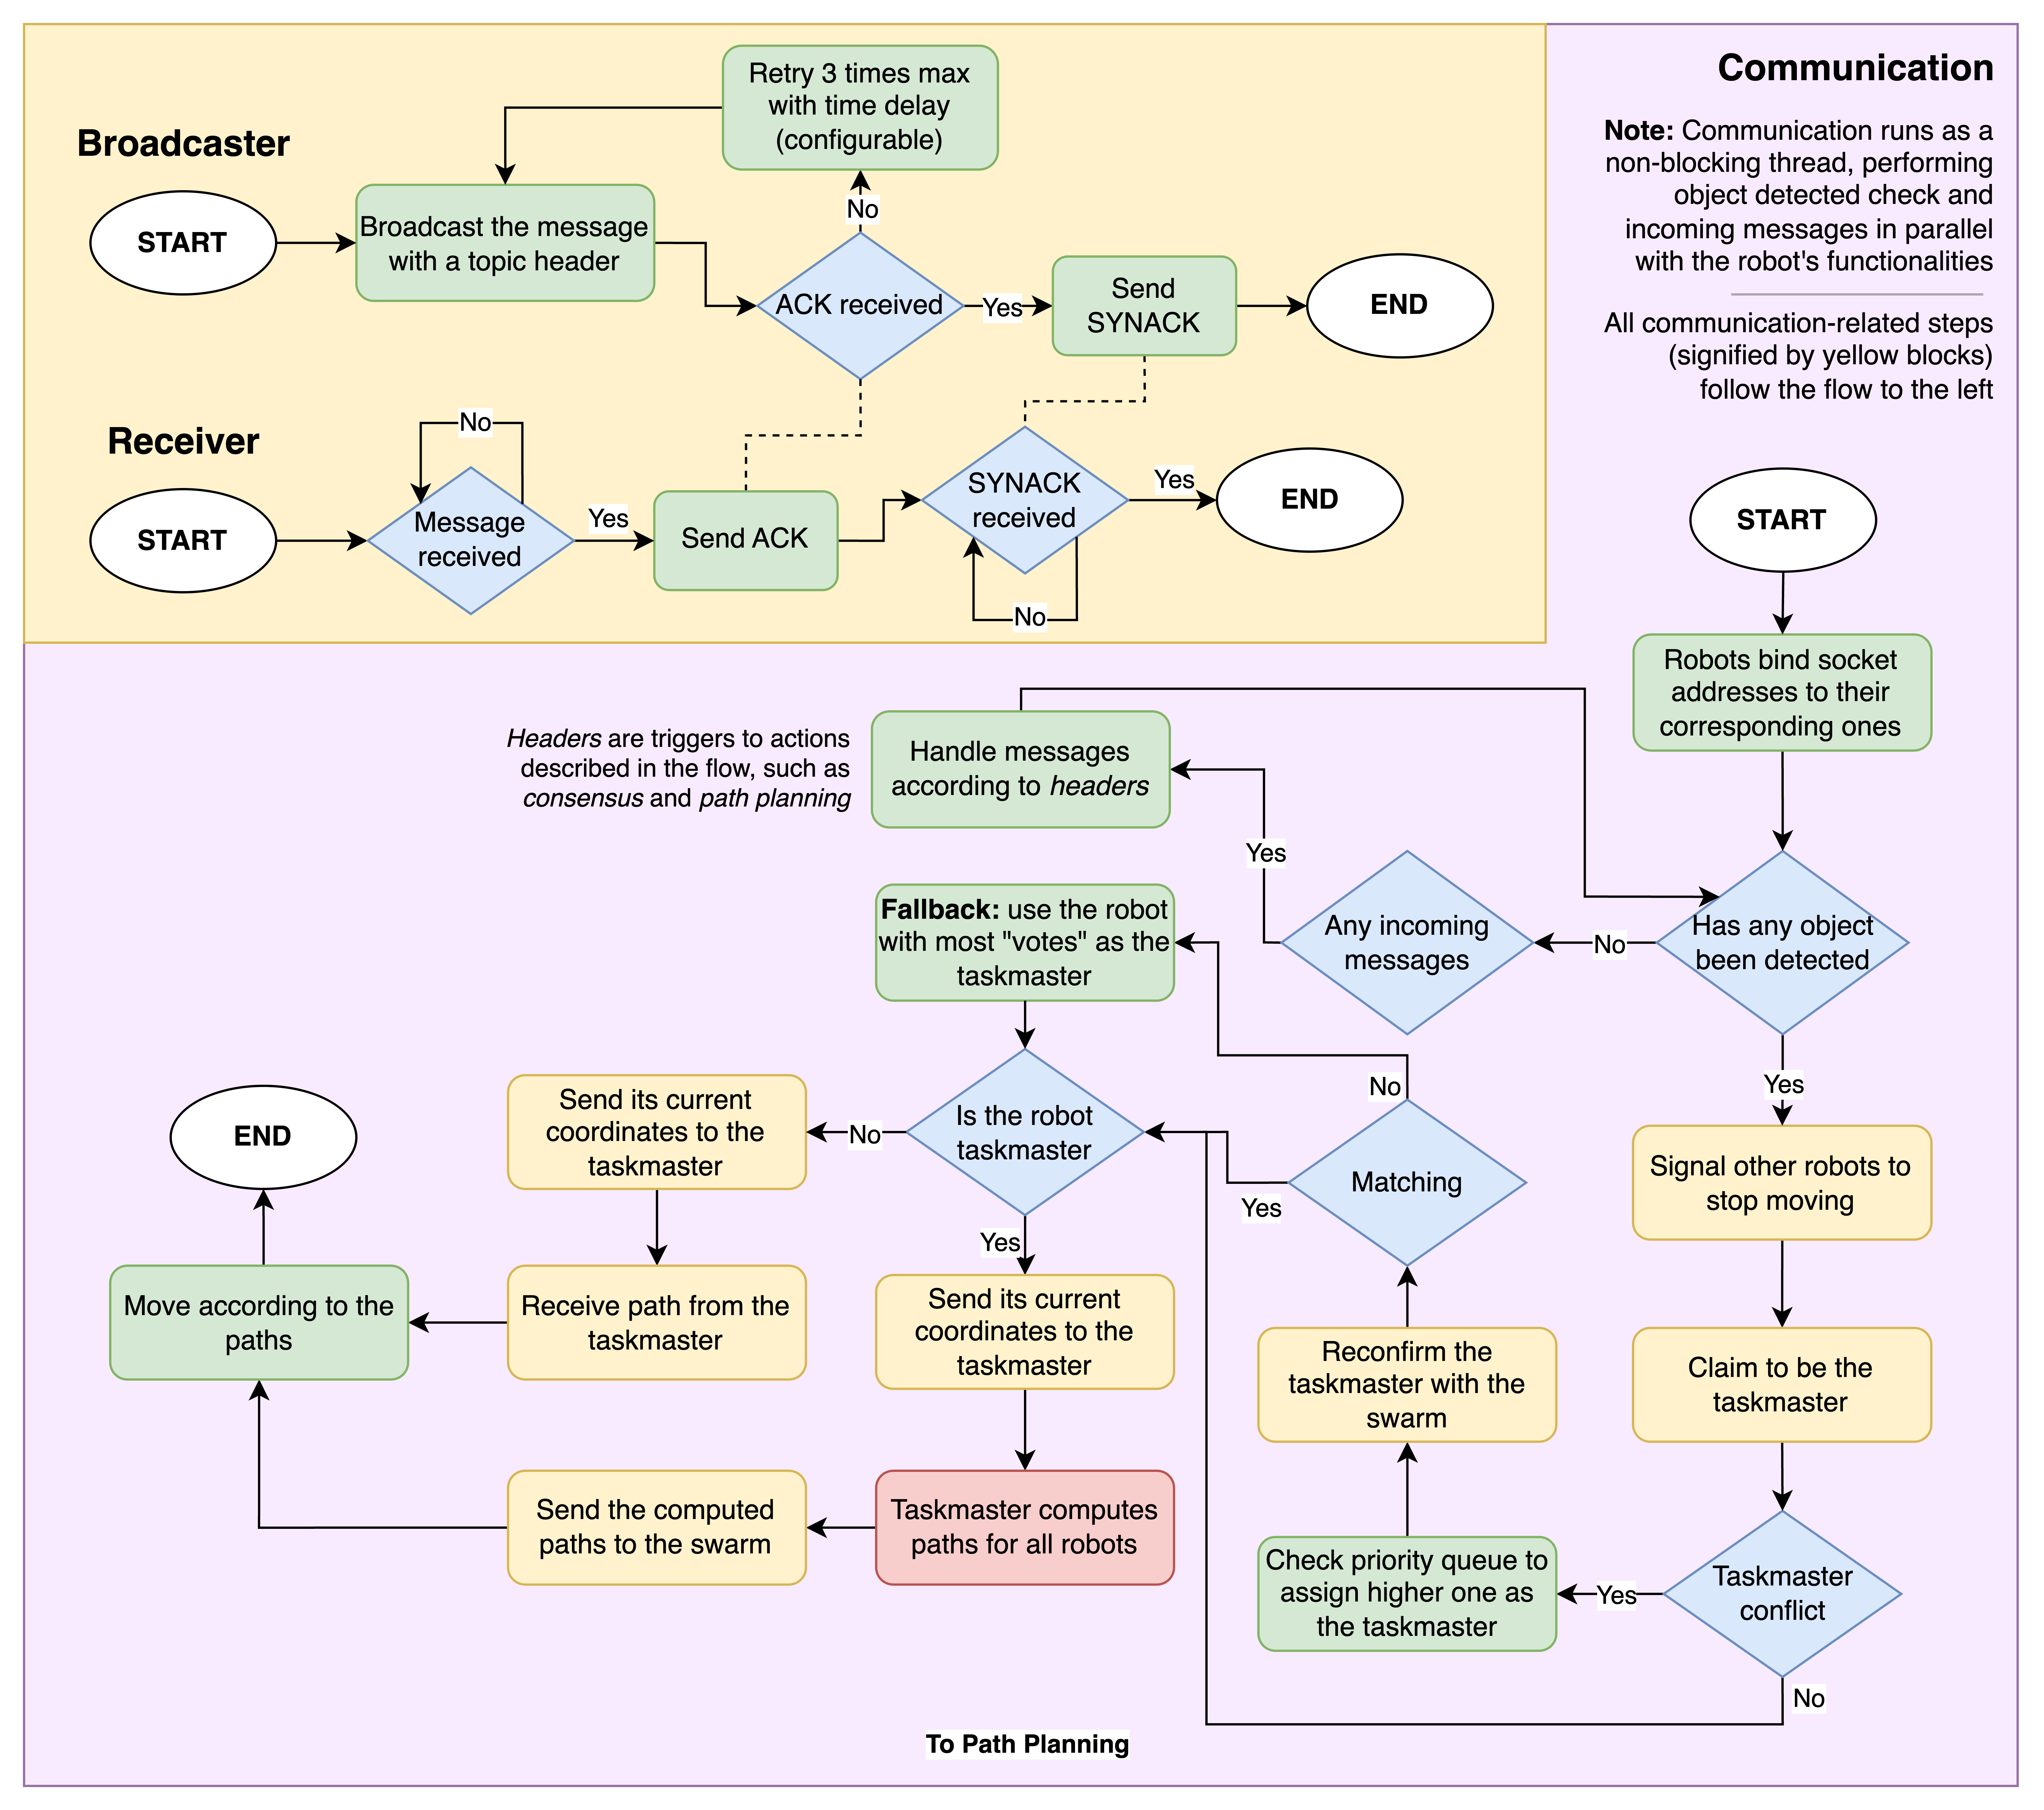
\includegraphics[width=0.85\linewidth]{assets/images/communication/communication-flow.png}
    \caption{Communication in the Swarm Detailed Flow}
    \label{fig:communication-flow}
\end{figure}

\paragraph*{}
There are two main implementations using communication mechanism in the swarm. The implementations are the \textbf{"constant coordinate stream"}, and the \textbf{"swarm detection task flow"}. For simplicity, all future descriptions of the communication mechanism will refer to the robots as \textit{"Robot A"}, \textit{"Robot B"} and \textit{"Robot C"}.

\paragraph*{}
The \textbf{constant coordinate stream} is a stream of coordinates in a fixed, configurable interval between the robots A, B, and C. They share their current X and Y positions with one another, updated by data obtained from the odometry. It is essential for the robots in the swarm to know the positions of one another so the movement controller will allow them roam in a collision-free manner. Figure \ref{fig:coordinate-stream} is a terminal output meant to provide an overview to the data the robots will obtain from this coordinate stream. The output is obtained from Robot C, where it is able to continuously track the coordinates of Robot A and Robot B, even with the others' coordinates being updated from their movement.

\begin{figure} [H]
    \centering
    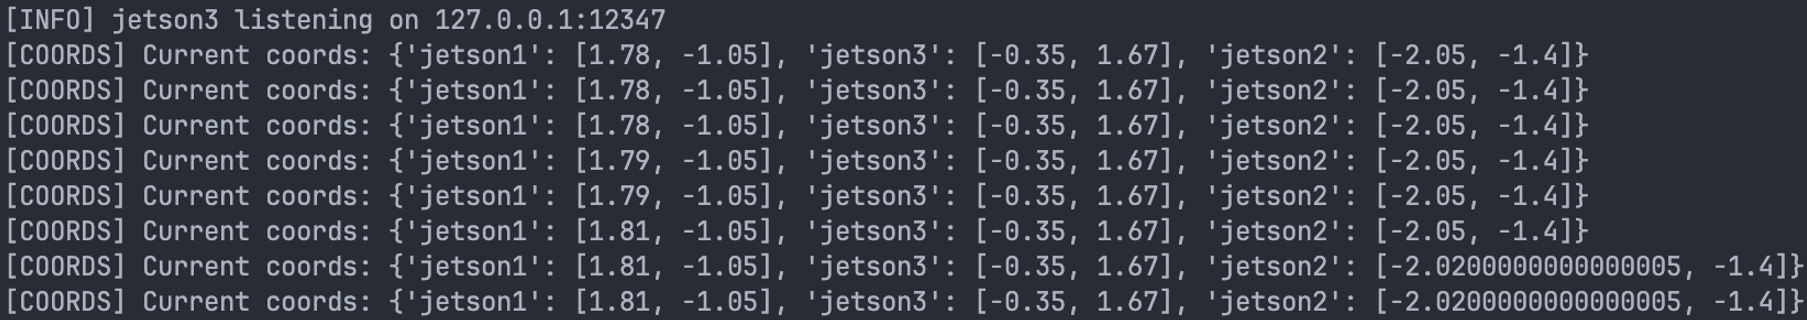
\includegraphics[width=1\linewidth]{assets/images/communication/coordinate-stream.png}
    \caption{Constant Coordinate Stream}
    \label{fig:coordinate-stream}
\end{figure}

\paragraph*{}
The other essential communication implementation is the \textbf{swarm detection task flow}. When an object gets detected by the robot's object detection, the detecting robot will send a signal to the other two robots to stop moving. In the example instance where Robot B claimed to be the taskmaster (Figure \ref{fig:example1-robot-b}), Robot A and Robot C receive a signal to stop ongoing movement (Figure \ref{fig:example1-robot-a}) and await a collisionless path to move towards the object by the swarm's path planning algorithm, detailed in a later chapter.

\paragraph*{}
The taskmaster, in this case, Robot B, will request current coordinates from Robot A and Robot C, then trigger the path planning algorithm for a set of collisionless paths for each robot. Once the set of paths are computed by the taskmaster, it will subsequently broadcast them towards others the swarm. In this case, Robot B performs the computation and broadcasts to Robot A and Robot C, allowing all of them to have a determined path to move towards the detected object (Figure \ref{fig:example1-robot-c})

\begin{figure} [H]
    \centering
    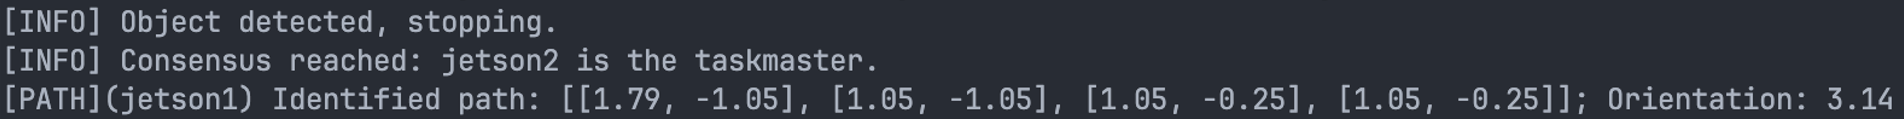
\includegraphics[width=1\linewidth]{assets/images/communication/example1-a.png}
    \caption{Example 1 - Robot A}
    \label{fig:example1-robot-a}
\end{figure}

\begin{figure} [H]
    \centering
    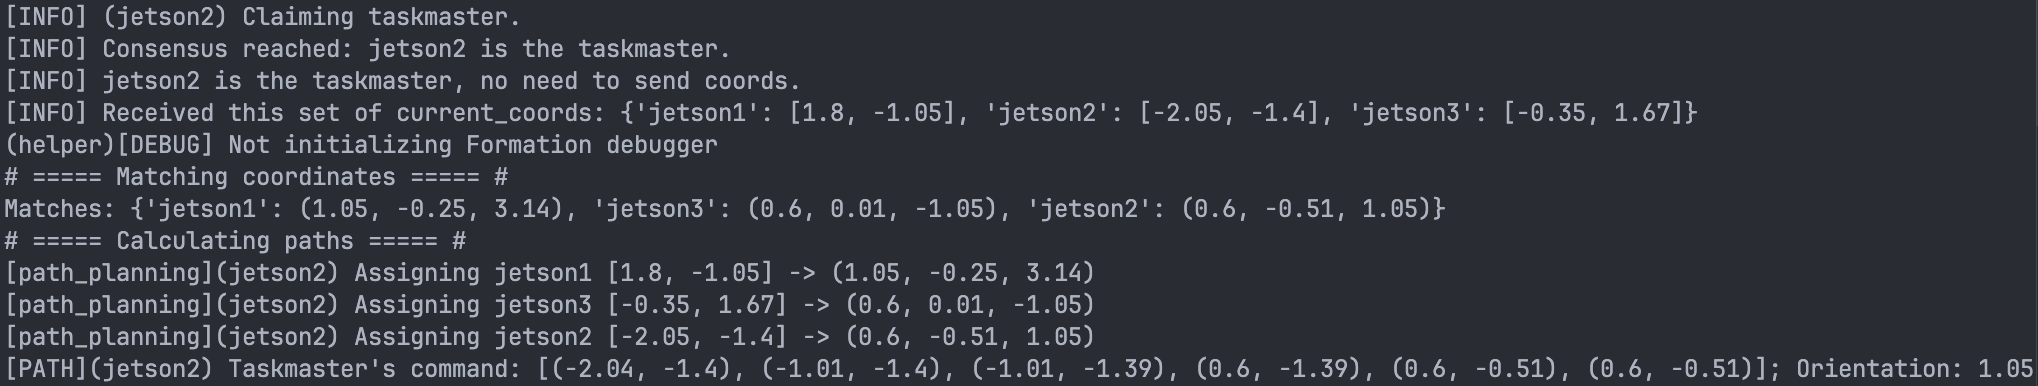
\includegraphics[width=1\linewidth]{assets/images/communication/example1-b-master.png}
    \caption{Example 1 - Robot B (Taskmaster)}
    \label{fig:example1-robot-b}
\end{figure}

\begin{figure} [H]
    \centering
    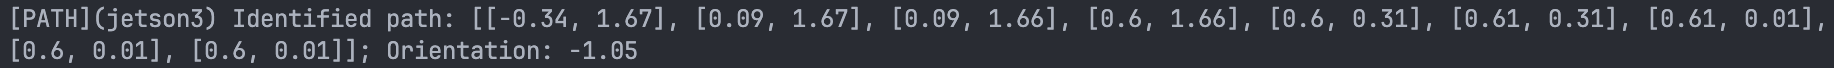
\includegraphics[width=1\linewidth]{assets/images/communication/example1-c.png}
    \caption{Example 1 - Robot C}
    \label{fig:example1-robot-c}
\end{figure}

\paragraph*{}
Another thing to note is that any swarm member can become the taskmaster and perform the computations according to the \textit{swarm detection task flow}. In Figure \ref{fig:example2-robot-a}, another claim for taskmaster had been made by Robot A, where the communication flow proceeded as expected. This was done after the initial swarm detection task flow in Figure \ref{fig:example1-robot-a}, \ref{fig:example1-robot-b}, and \ref{fig:example1-robot-c}, where Robot B claimed to be the taskmaster. This shows the versatility in the communication mechanism of the swarm. 

\begin{figure} [H]
    \centering
    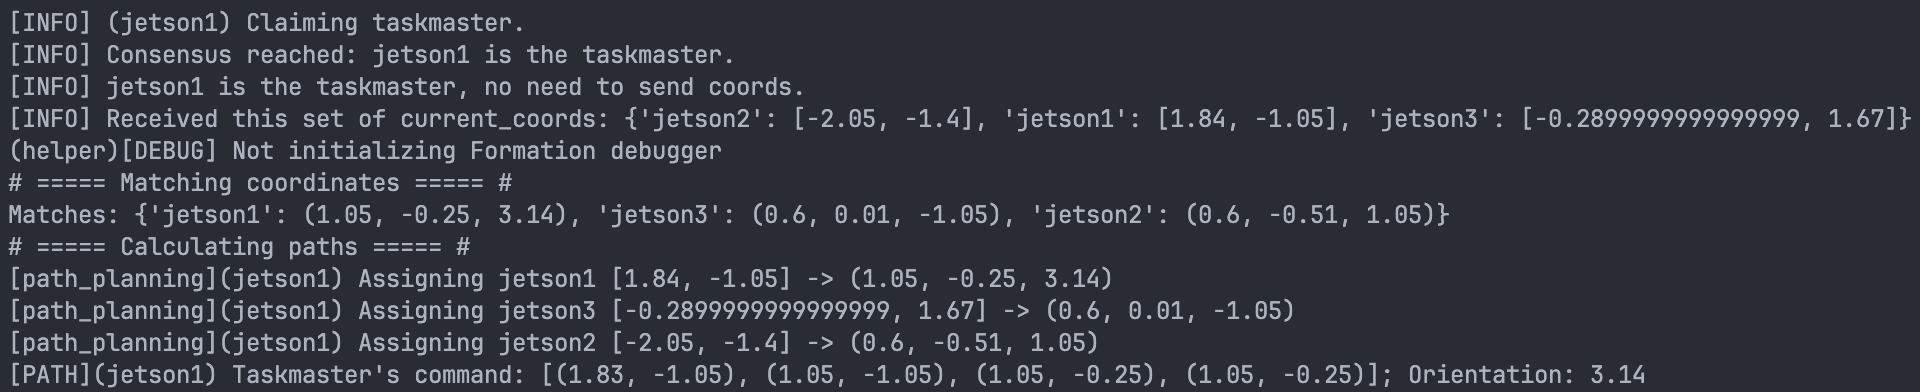
\includegraphics[width=1\linewidth]{assets/images/communication/example2-a-master.png}
    \caption{Example 2 - Robot A}
    \label{fig:example2-robot-a}
\end{figure}

\paragraph*{}
Since there is a claiming mechanism to become the taskmaster in charge of path computations, it is imperative to design communication in such a way that any \textit{conflicting claims} in the exact moment are handled appropriately. An instance of \textit{conflicting claims} is when multiple robots detect the object at the same time, hence claiming to become the taskmaster. The handler of this situation is the designed \textbf{consensus algorithm} for the swarm. Figure \ref{fig:consensus-algorithm} outlines the underlying mechanism of the consensus algorithm.

\begin{figure} [H]
    \centering
    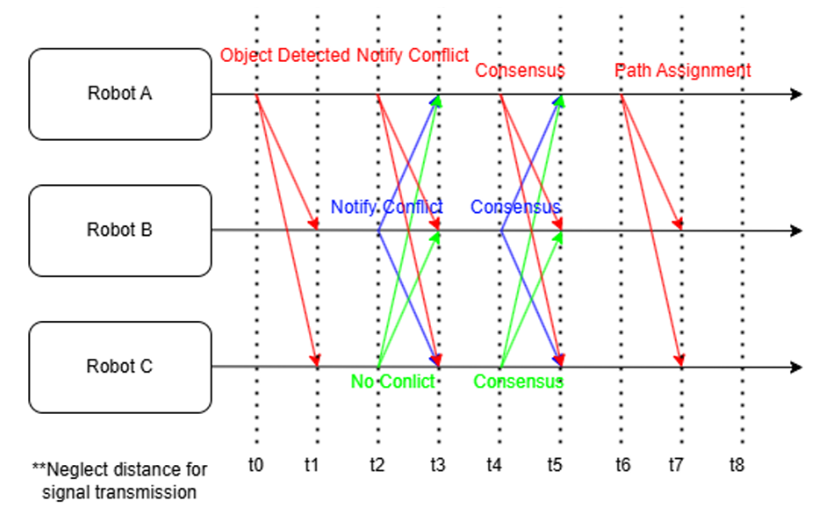
\includegraphics[width=0.9\linewidth]{assets/images/communication/consensus.png}
    \caption{Consensus Algorithm}
    \label{fig:consensus-algorithm}
\end{figure}

\paragraph*{}
The consensus algorithm functions by referring to a \textit{priority queue} once conflicting claims are observed. This priority queue determines the taskmaster by appointing the claimant with the higher priority the taskmaster role. Subsequently, the claimant is repositioned to the end of the priority queue for future claims to partially decentralize the operation. An account of this consensus mechanism is when Robot A and Robot C detect an object at the same time, with Robot C being higher on the priority queue. Robot C will get the taskmaster assignment for that particular detection, then rearranged to the end of the priority queue. If Robot A and Robot C detect an object at the same instance again, Robot A will receive the role, and also gets rearranged to the end of the queue. After the taskmaster assignment resolution is complete, the \textit{swarm detection task flow} will occur as designed.

\paragraph*{}
The approaches for communication in the swarm described above are all required mainly because the robots have to efficiently utilize available resources and coordinate to avoid collisions at all time. The \textit{constant coordinate stream} is to avoid collisions while in the state of random movement, in other words while no objects have been detected. The \textit{swarm detection task flow} is designed to efficiently travel to designated coordinates in order to prepare for collective movement of the detected object by gripping. The consensus algorithm is also designed to allow seamless coordination and eliminate potential conflicts in the swarm communication.
